
\documentclass[border=10pt]{standalone}
\usepackage{pgfplots}
\pgfplotsset{compat=1.18}
\begin{document}
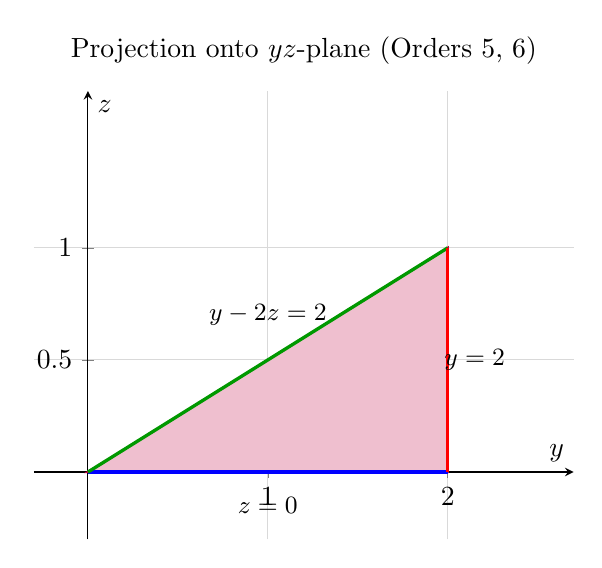
\begin{tikzpicture}
\begin{axis}[
    xmin=-0.3, xmax=2.7,
    ymin=-0.3, ymax=1.7,
    xlabel={$y$}, ylabel={$z$},
    title={Projection onto $yz$-plane (Orders 5, 6)},
    grid=major, grid style={gray!30},
    axis lines=middle,
    enlargelimits=false,
    xtick={0,1,2}, ytick={0,0.5,1},
]
% Filled triangle: (0,0), (2,0), (2,1)
\addplot[fill=purple!25, draw=purple, thick] coordinates {(0,0) (2,0) (2,1)} -- cycle;
\addplot[blue, very thick] coordinates {(0,0) (2,0)};
\node at (axis cs:1.0,-0.15) {\small $z=0$};
\addplot[green!60!black, very thick] coordinates {(0,0) (2,1)};
\node at (axis cs:1.0,0.7) {\small $y-2z=2$};
\addplot[red, very thick] coordinates {(2,0) (2,1)};
\node at (axis cs:2.15,0.5) {\small $y=2$};
\end{axis}
\end{tikzpicture}
\end{document}
